
%: ----------------------- introduction file header -----------------------
% the code below specifies where the figures are stored
\graphicspath{{4/figures/}}

\chapter{Timbre Similarity}
\label{chp:timbre}

Timbre is a difficult attribute to define in acoustic perception.
Research has long sought to better understand the latent dimensions, in the hope of developing methods that can estimate the pairwise similarity between observations.
In lieu of adequate information to study this phenomenon directly, here instrument taxonomies are used as an approach to objectively define such relationships.
A non-linear semantic embedding is achieved by training a deep convolutional network to project time-frequency representations of audio into a low-dimensional, semantically organized space.
The discriminative properties of the resulting embeddings are explored, and the notions of timbral smoothness are investigated qualitatively.


\section{Context}
\label{sec:context}

% Definition
Despite its common usage in the various forms of music for centuries, a satisfactory definition of \emph{timbre} remains elusive to this day; in fact, the one adopted by the American National Standards Institute embodies this challenge, arriving at a concept through the exclusion of others \cite{ANSI197x}:

\begin{quote}
Timbre is that attribute of auditory sensation in terms of which a subject can judge that two sounds similarly presented and having the same loudness and pitch are dissimilar.
\end{quote}

%  More focus on what it isn't than what it is
As evidenced by this definition, the very notion of ``timbre'' is still an open research topic in psychoacoustics.
This reality is captured quite succinctly by Phillipe Manoury, who offered the following insight \cite{}:

\begin{quote}
One of the most striking paradoxes concerning timbre is that when we knew less about it, it didn’t pose much of a problem.
\end{quote}

% Why is this problematic
There are many advantages to developing a deeper understanding of timbre, from both an artistic and scientific perspective.
Of particular interest to this work, however, the absence of a constructive definition ---timbre is a result of X, Y, and Z--- makes it difficult to directy build computational systems to characterize and compare timbres.
Thus, before proceeding, it is valuable to review what is known of timbre, and prior efforts to transfer this knowledge into engineering systems.
% There is much to be understood about "timbre"; point is, question everything we think we know.


\subsection{Psychoacoustics}
% Historical context
% Psychoacoustics, Early work and the struggle to define
% Helmholtz, pitch, and other psychoacoustics.
%Given this inherent ambiguity in concept definition, it is worthwhile to contextualize how this situation came to be.
The perception of timbre falls under the umbrella of \emph{psychoacoustics}, a topic of study that sits at the boundary between acoustics and psychology.
Some of the earliest research in psychoacoustics was pioneered by von Helmholtz in his inquiries into the sensations of pitch and loudness \cite{Cook1995?}.
Inquiries specific to timbre would not come until much later, due to two difficulties in experimental design.
One, whereas pitch and loudness are predominantly one dimensional, it is unclear from personal introspection what the salient dimensions of timbre might be.
A subject might describe a sound as being ``brighter'' than another, but signal analysis is necessary to begin to determine why.
Additionally, researchers were limited by the kinds of stimuli they could create and use in perceptual experimentation, and thus were constrained in the space of possible parameters to explore.

% Psychology and psychoacoustics in the 1960-90s
With the advent of computers and continued scientific advances through the 20th century, these issues could be addressed directly, and several researchers set out to identify the existence of fundamental dimensions.
This work, perfomed by Plomp \cite{Plomp1976} Grey and Wessel \cite{Grey1979}, among others, adopted a similar experimental design.
Human subjects were presented pairs of sound stimuli and asked to rate the pairwise similarity between the two.
Having collected a number of ratings from a number of participants, multi-dimensional scaling was used to project the stimuli into a low-dimesional space that preserved the given relationships.
At this point, the researcher would then turn to spectral analysis to identify possible charateristics of the stimuli that might correlate with the different dimensions of the resulting projection.
This approach proved relatively fruitful, yielding a variety of signal-level statistics, or \emph{features}, found to correspond positively with subjective ratings.
Conclusions drawn from this work suggested features such as log-attack time, spectral centroid, and spectral spread, and were echoed later, as in the work of Krumhansl \cite{}.
This line of inquiry showed promise, and went on to inform much of how MIR approaches timbre and how such systems should be built.

% Deficiencies
%  - at the mercy of researcher ingenuity to find good features
%  - subjective ratings are limited by the space of stimuli used
However, more recent work identifies two issues with this approach to timbre research \cite{Glennon2014}.
First, as stated by Caclin et al., ``Given the multiplicity of acoustical parameters that could be proposed to explain perceptual dimensions, one can never be sure that the selected parameters do not merely covary with the true underlying parameters.'' \cite{Caclin2005}.
This statement can be interpreted in two related ways:
one, the space of parameters considered is bounded by the insight and ingenuity of the researcher;
and two, it is possible that a chosen parameter covaries with the true, but unobserved, parameter.
Second, the utility of a timbre space resulting from MDS is limited to the space of stimuli with which it was obtained.
In other words, factors of variance not captured by the sonic palette used as stimuli are unlikely to be encoded in the resulting dimensions.

There is also a concern regarding the degree to which conclusions resulting from research on subjective pairwise ratings might be generalized.
Typically, stimuli used in such experiements are synthetic to the point of unnatural \cite{Teresawa2007?} or chosen from a space of instrument sounds.
In the latter case, familiarity with such sounds have the potential to bias subjects away from a purely perceptual rating.
Finally, the perpection of timbre undoubtedly has a time-varying characteristic, but much research focuses on timbre as a stationary phenomena.
Some, like \cite{Krumhansl1980?}, have considered the attack and sustained regions of a sound separately, finding that instrument identification was possible from either portion.
However, by concatenating the attack of one instrument with the sustained portion of another, it was demonstrated that a subject would perceive only the attack instrument, effectively masking the signature survived in the sustain.
Such a finding illustrates that the perception of timbre not only varies over small time scales, but is dependent on context and the sequential ordering of events.

%Synthesizing this brief survey of timbre perception research into some kind of workable defintion, timbre is a time-varying quality of sound, akin to texture in the visual domain.
% Referred to by Landy as a \emph{second-order percept}, texture is the emergent property

% What are the take-aways here?
% - Previous claims of salient dimensions should be taken with a grain of salt.
% - This is why we are where we are.


\subsection{Computational Modeling}
% Computational approaches and models
% Short-time statistics
Most previous approaches to computationally modeling timbre instantaneously can be grouped into one of two categories: signal statistics and basis projections.
The first follows from the perceptual research of the later 20th century, whereby statistics representing higher level concepts are computed for their semantic merit.
Initially these corresponded to the features named by in the work of Grey or Krumhansl, but have expanded over time to include a wide array of creative and clever measures.
The interested reader is directed to \cite{Essid2006} for a comprehensive space of possible features.


% Cascaded Transforms
From an often complimentary perspective, other music researchers have designed transform-based systems to project signals into representations with various properties.
One of the earliest and most common approaches is the use of Mel-frequency Cepstral Coefficients (MFCCs) for timbre-oriented tasks.
Originally designed for speech coding purposes by Mermelstein in the 1960s \cite{Mermelstein}, the first significant contribution in MIR to call attention to these features was that of Logan in 2000 \cite{Logan}.
MFCCs have, if not in reality then at least in practice, become synonymous with timbre-centric MIR, now being used in an innumerable number of systems for instrument classification \cite{}, tagging \cite{}, genre prediction \cite{}, mood estimation \cite{} or structural analysis \cite{}, to name only a few representative works in each.
The general process of computing MFFCs is given in Figure and proceeds as follows: an input audio signal is divided into overlapping, short-time \emph{frames}, on the order of tens to hundreds of milliseconds; a filterbank, perceptually scaled in frequency, is then applied to each short-time frame and log-compressed; finally, a discrete cosine transform (DCT) is applied to these frequency coefficients, characterizing the shape of the spectrum (or the spectrum of the spectrum, referred to rather cheekily as the \emph{ceps}trum).
Often only the first dozen or so coefficients are used in practice on the principle that they capture the most relevant information, though this is more convention than rule.

% Machine learning approaches
Similar in principle, though less widely used, is to instead \emph{learn} the set of bases over which the spectrum is projected.
For exaple, the approach taken by Jehan \cite{Jehan2005}, which preserves the first 12 coefficients of a trained PCA decomposition.
In this instance, the projection into the PCA subspace attempts to decorrelate the principal axes of the data in the input space, like the Discrete Cosine Transform.
The primary difference here, however, is that the bases are learned from a sample of observations.

\subsection{Motivation}

% Motivation for similarity
While many of these approaches have proven useful in various classification tasks, none directly result in a notion of timbre similarity, a useful concept in a variety of scenarios.
The search and navigation of large sound libraries is one such instance, where sparse metadata and text-based queries often reduce the task of navigating a sound library to that of an exhaustive, brute force search.
The inherent difficulty of finding a target sound in a potentially massive collection of items lies in the inability to capture the specific query semantically, relying instead on metaphors; distorted guitars are described as `crunchy' or trumpets `bright.'

User interfaces
Composition and

\subsection{Limitations}
Failing to adopt a clear definition of timbre does not relieve you of inherently operating on one.
The work presented here is not intended to be synonomous with timbre, and is subject in many ways to the limitations named in previous perceptual research; a timbre space is achieved as a result of the inputs considered, and will likely fail on sufficiently novel stimuli.
% Additionally, you can't learn everything.


\section{Learning Timbre Similarity}
\label{sec:timbre_embedding}

From the previous review of psychoacoustics research and efforts to computationally model timbre, there are two important conclusions to draw:
first, classic timbre features are subject to the wisdom that ``corellation does not imply causation'';
and second, these features are ultimately bounded by the creativity, insight, or dilligence of a researcher.
Synthesizing these observations with the discussion from Chapter \ref{chapter:context}, there is a clear argument for feature learning in timbre-related tasks.

Having discussed the value and applications of a timbre similarity space, it is worthwhile to outline the goals for such a system.
First and foremost, one would learn, rather than design, signal-level features relevant to achieve the given task and circumvent the issues identified previously.
% This idea is based on the combination of an inability to clearly define the sensory phenomenon and the known caveats of previous perceptual studies.
Additionally, sound should be represented in an intuitive manner, such that distance between points is semantically meaningful.
In other words, signals from the same source should be near-neighbors, whereas sounds from different sources should be far apart.
% Come back to how we show this in the methodology.
Finally, the ideal similarity space is perceptually \emph{smooth}, meaning that a point that interpolates the path between two others should be a blend of the two, e.g. a tenor saxophone might fall between a clarient and a French horn.

These objectives have clear conceptual overlap with dimensionality reduction methods and instrument classification systems, on which this work builds.
In lieu of precise information regarding the relationship between two given sounds, music instrument classes are used as a proxy for timbre similarity.
The approach presented here consists of several parts, as diagrammed in Figure \ref{fig:nlse}, and discussed in the following subsections.
First, all audio is transformed into a time-frequency representation (Subsection \ref{subsec:timbre_tfr}).
The main component of the system is a deep convolutional network, which maps tiles of these time-frequency coefficients into a low-dimensional space (Subsection \ref{subsec:timbre_deepnet}).
A pairwise training harness is made by copying this network, and parameters are learned by minimizing the distance between observations of the same sound source and maximizing the distance otherwise (Subsection \ref{subsec:timbre_pairwise}).
At test time, the pairwise harness is discarded, and the resulting network is used to project inputs to the learned embedding space.


\subsection{Time-Frequency Representation}
\label{subsec:timbre_tfr}

Though it is a particular goal of the system to minimally design transformations, audio is first processed by a Constant-Q transform (CQT) for three reasons.
First, the application of a filterbank front-end results in a considerable simplification of the system, both computationally and in the number of learned parameters.
Sharing a common formulation with neural networks, a filterbank can be viewed as a hard-coded layer in the network.
Knowing the parameters in advance allows for the development of an optimized implementation, such as the one discussed in Chapter \ref{chapter:deep_learning}, reducing processing time.
Additionally, the CQT is logarithmic in frequency, serving as a reasonable approximation of the human auditory system.
Furthermore, it is generally agreed upon that timbre perception is, at least to some degree, invariant to pitch.
Also following from this earlier discussion, the use of convolutional networks allows for translation invariance of features in both $log_2$-frequency and time.

The constant-Q filterbank is parameterized as follows: all input audio is first downsampled to 16kHz; bins are spaced at 24 per octave, or quarter-tone resolution, and span eight octaves, from 27.5Hz to 7040Hz; analysis is performed at a framerate of 20Hz uniformly across all frequency bins.
Logarithmic compression is applied to the frequency coefficients with an offset of one, e.g. $log_{1p}(x) = log(x + 1.0)$.


\subsection{Deep Convolutional Networks for Timbre Embedding}
\label{subsec:timbre_deepnet}

Noting that the details of deep learning and convolutional networks are discussed at length previously, only those decisions unique to this task are addressed here; for clarity regarding the mathematical or conceptual definitions of these terms, refer to Chapter \ref{chapter:deep_learning}.

A five-layer neural network is designed to project time-frequency inputs into a low-dimensional embedding.
The first three layers make use of 3D-convolutions, to take advantage of translation invariance, reduce the overall parameter space, and act as a constraint on the learning problem.
Max-pooling is applied in time and frequency, to further accelerate computation by reducing the size of feature maps, and allowing a small degree of scale invariance in both directions.
The final two layers are fully-connected affine transformations, the latter of which yields the embedding space.
The first four hidden layers use a hyperbolic tangent as the activation function, while the visible output layer is linear, i.e. it has no activation function in the conventional sense.

Hyperbolic tangents are chosen as the activation function for the hidden layers purely as a function of numerical stability.
It was empirically observed that randomly initialized networks designed with rectified linear units instead were near impossible to train; it is hypothesized that, due to the relative nature of the learning problem, i.e. the network must discover an equilibrium for the training data, it is easy for the parameters to be pushed into a space where all activations go to zero, collapsing the network.
Conversely, hyperbolic tangents are everywhere-differentiable, and did not suffer the same behavior.
The use of activation functions that provide an error signal everywhere, such as sigmoids or ``leaky'' rectified linear units \cite{Maas2014}, or better parameter initialization might avoid this behavior, but neither were explored here.

Combining the successful application of linear ``bottleneck'' layers \cite{Liao2013} with lessons learned from previous efforts \cite{Humphrey2011}, the visible layer is chosen here to be linear.
As will be discussed in more detail shortly, a saturating nonlinearity at the output makes the choice of hyperparameters crucial in order to prevent the network from pushing datapoints against the limits of its space.
However, the absence of boundaries allows the network to find the appropriate scale factor for the embedding.

Specifically, the network is parameterized thusly: the input to the network is a
2D tile of log-CQT coefficients with shape $(20, 192)$, corresponding to time
and frequency respectively; the first convolutional layer uses 20 filters with
shape $(1, 5, 13)$ and max-pooling with shape $(2, 2)$; the second convolutional
layer uses 40 filters with shape $(20, 5, 11)$ and max-pooling with shape $(2,
2)$; the third convolutional layer uses 80 filters with shape $(1, 1, 9)$ and
max-pooling with shape $(2, 2)$; the fourth layer is fully-connected and has 256
outputs; the final layer is also fully connected, and has 3 outputs.


\subsection{Pairwise Training}
\label{subsec:timbre_pairwise}

% Relative vs absolute
As discussed previously, there are currently no known quantities with which to measure timbre, in the same way that fundamental frequency has Hertz or loudness decibels.
In the absence of this absolute reference, previous efforts have instead tried to determine the relative relationships between a collection of observations.
Collecting this data subjectively quickly becomes prohibitive, as the number of pairwise comparisons to be made increases quadradically with the total number of observations considered.
Music instruments, however, provide an interesting source of objective information for this problem.
Based on the coarse approximation that all sounds produced by a single instrument are in some sense similar, regardless of pitch or loudness, class boundaries can be used to define a neighborhood of similar timbres.

% TODO-future: Don't tie everything together, just pick k-NN from *inside* the one class, should be smoother
% TODO-future: Explore soft similarity scores rather than binary values
This approach to defining timbre ``neighborhoods'' can be used to extend the work of Hadsell et al \cite{Hadsell2007} to address this challenge of learning a timbre similarity space.
Referred to by the authors as ``dimensionality reduction by learning an invariant mapping'' (DrLIM), a deep network was trained in a pairwise manner to minimize the distance between ``similar'' data points in a learned, nonlinear embedding space, and vice versa.
Similarity was determined in an unsupervised manner by linking the $k$-nearest neighbors in the input space.
Though left as future work, the authors propose that other information, such as class relationships, might be levereaged to learn different embeddings.
This is an important consideration for the problem of timbre, because fundamental frequency and amplitude are likely to dominate the graph of nearest neighbors in the input space.

The intution behind DrLIM is both simple and satisfying: datapoints that are deemed ``similar'' should be close together, while those that are ``dissimilar'' should be far apart.
Though the precise distance metric is a flexible design decision, it is used here in the Euclidean sense.
A collection of similar and dissimilar relationships can be viewed as a physical system of attractive and repulsive forces.
Learning proceeds by finding a balance of these contrasting forces; and furthermore, this analogy illustrates the need for both positive and negative forces to maintain equilibrium.

% This first sentence blows, come back to this.
At its core, DrLIM is ultimately a pairwise training strategy.
First, a parameterized, differentiable function, $f(\dot | \Theta)$, e.g. a neural network, is designed for a given problem; for the purposes of dimensionality reduction, the output will be much smaller than the input, and typically either 2 or 3 for the purposes of visualization.
During training, the function $f$ is copied and parameters, $\Theta$, \emph{shared} between both, such that $f_1(\dot | Theta) == f_2(\dot | Theta)$.
Two inputs, $X_1$ and $X_2$, are transformed by their respective functions, $f_1$ and $f_2$, to produce the outputs, $Z_1$ and $Z_2$.
A metric, e.g. Euclidean, is chosen to compute a distance, $D$ between these outputs.
Finally, a similarity score, $Y$, representing the relationship between $X_1$ and $X_2$, is passed to a contrastive loss function, which penalizes similar and dissimilar pairs differently.
When the pair is similar, the loss will be small when the distance is small; for dissimilar pairs, the loss will be small when the distance is outside a given margin, $m$.
This is expressed symbolically by the following:


\begin{equation}
Z_1 = f_1(X_1 | Theta), Z_2 = f2(X_2 | Theta)\\
D = || Z_1 - Z_2 ||_2\\
\mathcal{L} = Y * D^2 + (1 - Y) * max(0, m - D)^2\\
\end{equation}

\noindent~Note that similarity is given by $Y=1$, for consistency with boolean logic.
As a result, the first term of the loss function is only non-zero for similar pairs, and the inverse is true for the second term.

%Training strategy
Returning to the previous discussion regarding the dynamic range of the output layer, it should now be clear that the choice of margin only influences the learned embedding relative to a scale factor when the output is unbounded.
The two loss terms are mirrored parabolas, and changing the margin, or horizontal offset, only serves to move the vertical line at which they reflect, and not the curvature of the space.
In fact, this observation encourages a simple generalization of this loss function, where a second margin is introduced:

\begin{equation}
\mathcal{L} = Y * max(0, D - m_{sim})^2 + (1 - Y) * max(0, m_{diff} - D)^2 \\
\end{equation}

This generalized square-square loss is shown in Figure \ref{fig:double_margin} for various margin values.
Whereas the differential margin controls the variance of all points in space, the similar margin will control the variance of a similarity neighborhood.
In the original formulation, where implicitly $m_{sim} = 0$, the loss is lowest when all inputs are mapped to \emph{exactly} the same point; for the purposes of similarity, a more diffuse distribution of points is desirable.
It is worth noting the slight parallel to linear discriminant analysis, which seeks to minimize intraclass variance and maximize interclass variance.
Given the relative nature of this trade-off, it is sufficient to pick a single ratio between the margins, eliminating the need to vary both hyperparameters.


In practice, training proceeded via minibatch stochastic gradient descent with a constant learning rate, set at 0.02 for 25k iterations, or until a batch returned a total loss of zero.
Batches consisted of 100 comparisons, drawn such that a datapoint was paired with both a positive and negative example.


\section{Experimental Methodology}
\label{sec:example}

Here's the explanation of what was done.
What are the questions we want to address?

\begin{enumerate}
\item What is the effect of using different margin ratios?
\item How does this approach compare to other methods?
\item How does the set of instruments considered impact the learned embedding?
\item How perceptually ``smooth'' is the resulting space?
\end{enumerate}


\subsection{Data}
Start with the VSL
Use instrument boundaries as a nearest neighbor taxonomy.
Cut-off at 5000 sound files.
After discarding unreasonable duplicates, left with 24 classes.
Keep three conditions from the pilot study (c5, c8, c12), and one with all 24 classes.

\begin{figure}[h]
\centering
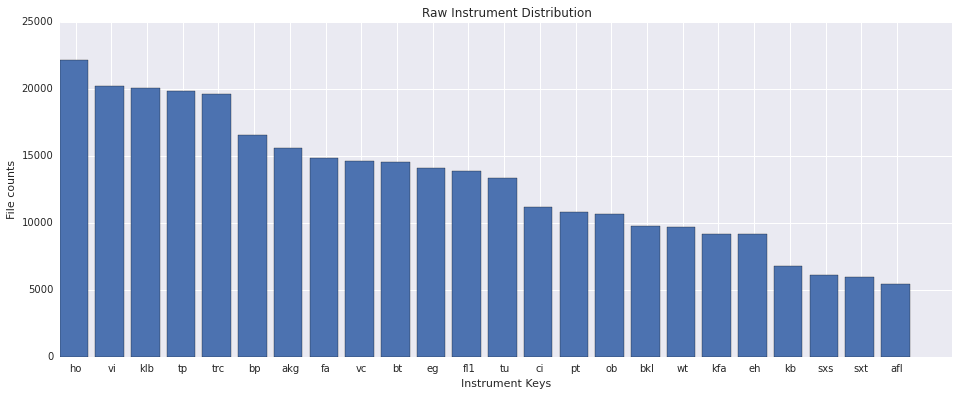
\includegraphics[width=\textwidth]{raw_vsl_distribution.png}
\caption{Raw distribution of instrument samples in the Vienna Symphonic Library.}
\label{fig:muffin}
\end{figure}


\begin{equation}
\nabla^2p = \frac{1}{c^2} \frac{\partial^2 p}{\partial t^2}
\label{eq:wave}
\end{equation}

Muffin dragee caramels sweet pudding danish bonbon jelly-o \gls{tcap}.
Dessert chocolate bar marzipan.
Tiramisu cheesecake caramels cake lemon drops. Icing pastry lollipop marshmallow jujubes.
Gingerbread carrot cake marzipan souffle halvah. Bear claw cheesecake toffee pie donut.
Dessert pastry applicake biscuit caramels marzipan croissant muffin \ref{tab:things}.

\begin{table*}[h]
\begin{center}
\caption{Instruments considered and their corresponding codes.}
\begin{tabular}{l | c || l | c}
Instrument & Code & Instrument & Code \\

\hline
French Horn & ho & Tuba & tu\\
Violin & vi & Cimbasso & ci \\
B$\flat$ Clarinet & klb & Piccolo & pt \\
Tenor Trombone & tp & Oboe & ob \\
C Trumpet & trc & Bass Clarinet & bkl \\
Bass Trombone & bp & Wagner Tuba & wt \\
Acoustic Concert Guitar & akg & Contra Bassoon & kfa \\
Bassoon & fa & English Horn & eh \\
Cello & vc & Bass & kb \\
Bass Trumpet & bt & Soprano Saxophone & sxs \\
Distorted Guitar & eg & Tenor Saxophone & sxt \\
Flute & fl & Alto Flute & afl \\

\hline
\end{tabular}
\label{tab:things}
\end{center}
\end{table*}



\begin{table*}[h]
\begin{center}
\caption{Instrument set configurations.}
\begin{tabular}{l | l }
Key & Instrument Codes \\
\hline

c5 & tu, ob, klb, vc, fl \\
c8 & trc, ho, ob, eh, klb, sxt, vi, vc \\
c12 & c8 + \{tp, tu, fa, fl\} \\
c24 & c12 + \{bp, akg, bt, eg, ci, pt, bkl, wt, kfa, kb, sxs, afl\} \\

\hline
\end{tabular}
\label{tab:things}
\end{center}
\end{table*}




\noindent
Icing cheesecake biscuit pudding marshmallow.
Cake toffee fruitcake gummi bears.
Macaroon macaroon lollipop marzipan.
Ice cream tiramisu pie powder halvah.





%train
\begin{table*}[h]
\begin{center}
\caption{k-Neighbors classification results over the training set.}
\small
\begin{tabular}{rllll}
 model \textbackslash config  & c5    & c8   & c12  & c24  \\
\hline
 0    & $93.81\pm0.53$ & $89.97\pm0.40$ & $86.70\pm0.39$ & $74.17\pm0.79$ \\
 0.25 & $94.21\pm0.18$ & $90.25\pm0.54$ & $87.17\pm0.35$ & $73.91\pm0.61$ \\
 0.5  & $93.04\pm0.29$ & $89.16\pm0.27$ & $86.08\pm0.26$ & $71.59\pm0.88$ \\
 \hline
 PCA-LDA & $64.44\pm0.47$ & $56.58\pm0.60$ & $47.22\pm0.45$ & $35.81\pm0.28$ \\

\hline
\end{tabular}
\label{tab:things}
\end{center}
\end{table*}

%valid
\begin{table*}[h]
\begin{center}
\caption{k-Neighbors classification results over the validation set.}
\small
\begin{tabular}{rllll}
\hline
model \textbackslash config & c5  & c8 & c12   & c24     \\
\hline
 0    & $92.37\pm0.64$ & $87.94\pm0.45$ & $84.52\pm0.97$ & $70.86\pm1.51$ \\
 0.25 & $93.75\pm0.53$ & $88.62\pm0.58$ & $85.65\pm0.26$ & $71.46\pm0.63$ \\
 0.5  & $91.75\pm0.67$ & $87.78\pm0.85$ & $83.78\pm0.53$ & $66.37\pm1.69$ \\
 \hline
 PCA-LDA & $59.97\pm0.96$ & $52.49\pm2.68$ & $39.25\pm2.01$ & $24.32\pm0.97$ \\
\hline
\end{tabular}
\label{tab:things}
\end{center}
\end{table*}


%test
\begin{table*}[h]
\begin{center}
\caption{k-Neighbors classification results over the testing set.}
\small
\begin{tabular}{rllll}
\hline
model \textbackslash config & c5  & c8  & c12   & c24   \\
\hline
 0    & $92.49\pm0.41$ & $88.26\pm0.74$ & $84.35\pm0.41$ & $70.67\pm0.55$ \\
 0.25 & $92.97\pm0.41$ & $88.67\pm0.79$ & $85.16\pm0.24$ & $70.28\pm0.86$ \\
 0.5  & $91.96\pm0.35$ & $87.83\pm0.25$ & $84.04\pm0.57$ & $66.91\pm0.57$ \\
 \hline
 PCA-LDA  & $59.91\pm0.77$ & $50.24\pm1.52$ & $39.32\pm0.86$ & $24.77\pm0.51$ \\
\hline
\end{tabular}
\label{tab:things}
\end{center}
\end{table*}


\begin{table*}[h]
\begin{center}
\caption{Confusion Matrix -- (c12, ratio=0.0).}
\scriptsize
\begin{tabular}{ccccccccccccc}
\hline
   & eh &    fa &   fl &    ho &   klb &    ob &   sxt &    tp &   trc &    tu &    vc &    vi \\
\hline
eh &  \textbf{84.96} &  0.65 &  0.76 &  1.41 &  1.43 &  5.73 &  1.52 &  0.33 &  2.60 &  0.22 &  0.47 &  1.09 \\
fa &   1.65 & \textbf{84.30} &  0.08 &  3.98 &  0.25 &  0.37 &  1.19 &  0.90 &  0.95 &  4.04 &  2.31 &  0.54 \\
fl &   0.88 &  0.17 & \textbf{85.42} &  0.71 &  2.56 &  3.65 &  3.24 &  0.13 &  1.57 &  0.23 &  0.51 &  0.75 \\
ho &   0.93 &  2.21 &  0.10 & \textbf{80.74} &  0.20 &  0.30 &  0.79 &  9.28 &  2.59 &  3.57 &  0.53 &  0.65 \\
klb &   1.02 &  0.12 &  1.52 &  0.64 & \textbf{85.38} &  4.93 &  3.46 &  0.12 &  1.01 &  0.31 &  2.30 &  0.54 \\
ob &   2.67 &  0.16 &  2.92 &  0.87 &  1.74 & \textbf{83.02} &  0.63 &  0.12 &  4.06 &  0.16 &  0.16 &  1.33 \\
sxt &   0.29 &  0.36 &  0.80 &  0.37 &  1.56 &  0.34 & \textbf{85.60} &  0.10 &  0.94 &  1.37 &  4.70 &  2.27 \\
tp &   0.51 &  0.45 &  0.06 & 10.97 &  0.06 &  0.34 &  0.46 & \textbf{78.47} &  2.73 &  2.79 &  0.54 &  0.45 \\
trc &   1.54 &  0.07 &  1.11 &  2.63 &  0.51 &  4.60 &  1.37 &  3.33 & \textbf{83.58} &  0.43 &  0.33 &  1.57 \\
tu &   0.19 &  2.31 &  0.05 &  4.02 &  0.13 &  0.11 &  1.51 &  2.36 &  0.56 & \textbf{84.69} &  3.27 &  0.32 \\
vc &   0.44 &  0.50 &  0.19 &  0.50 &  0.84 &  0.29 &  3.46 &  0.17 &  0.43 &  2.23 & \textbf{90.56} &  0.70 \\
vi &   0.81 &  0.31 &  0.65 &  1.48 &  0.43 &  1.59 &  5.06 &  0.56 &  2.17 &  0.51 &  1.97 & \textbf{85.23} \\
\hline
\end{tabular}
\label{tab:things}
\end{center}
\end{table*}


\begin{table*}[h]
\begin{center}
\caption{Confusion Matrix -- (c12, ratio=0.25).}
\scriptsize
\begin{tabular}{ccccccccccccc}
\hline
   & eh &    fa &   fl &    ho &   klb &    ob &   sxt &    tp &   trc &    tu &    vc &    vi \\
\hline
eh & \textbf{85.52} &  1.10 &  0.46 &  3.05 &  1.76 &  3.05 &  0.44 &  0.23 &  2.53 &  0.30 &  0.51 &  1.64 \\
fa &   1.74 & \textbf{85.82} &  0.05 &  3.93 &  0.26 &  0.19 &  0.63 &  0.81 &  0.51 &  3.64 &  2.48 &  0.51 \\
fl &   0.80 &  0.10 & \textbf{85.20} &  0.90 &  2.19 &  6.00 &  1.67 &  0.14 &  2.33 &  0.07 &  0.33 &  1.17 \\
ho &   0.76 &  1.88 &  0.07 & \textbf{82.52} &  0.26 &  0.29 &  0.33 &  6.50 &  1.18 &  2.73 &  0.88 &  1.26 \\
klb &   1.23 &  0.40 &  2.46 &  1.16 & \textbf{86.57} &  3.02 &  1.80 &  0.11 &  1.01 &  0.25 &  1.37 &  1.05 \\
ob &   2.90 &  0.06 &  3.09 &  1.12 &  2.56 & \textbf{81.22} &  0.44 &  0.17 &  5.29 &  0.04 &  0.04 &  1.39 \\
sxt &   0.24 &  0.38 &  1.01 &  0.51 &  1.24 &  0.84 & \textbf{86.34} &  0.14 &  0.48 &  0.65 &  4.97 &  2.78 \\
tp &   0.39 &  0.87 &  0.10 & 11.87 &  0.03 &  0.49 &  0.20 & \textbf{80.96} &  2.38 &  2.73 &  0.95 &  0.59 \\
trc &   1.14 &  0.11 &  1.77 &  3.84 &  0.56 &  4.13 &  0.59 &  1.74 & \textbf{83.45} &  0.08 &  0.09 &  2.47 \\
tu &   0.04 &  1.55 &  0.04 &  5.32 &  0.04 &  0.01 &  0.57 &  2.18 &  0.09 & \textbf{86.44} &  2.82 &  0.57 \\
vc &   0.27 &  0.53 &  0.24 &  1.51 &  0.79 &  0.49 &  2.68 &  0.27 &  0.63 &  2.32 & \textbf{89.74} &  1.49 \\
vi &   0.49 &  0.23 &  0.61 &  2.44 &  0.46 &  1.20 &  2.46 &  0.48 &  2.05 &  0.41 &  2.06 & \textbf{87.32} \\
\hline
\end{tabular}
\label{tab:things}
\end{center}
\end{table*}

\begin{table*}[h]
\begin{center}
\caption{Confusion Matrix -- (c12, ratio=0.5).}
\scriptsize
\begin{tabular}{ccccccccccccc}
\hline
  &  eh &    fa &   fl &    ho &   klb &    ob &   sxt &    tp &   trc &    tu &    vc &    vi \\
\hline
 eh & \textbf{83.85} &  1.13 &  0.56 &  2.70 &  2.05 &  3.89 &  0.67 &  0.27 &  2.35 &  0.20 &  0.78 &  1.55 \\
 fa &  1.59 & \textbf{83.41} &  0.03 &  5.87 &  0.36 &  0.07 &  0.51 &  0.50 &  0.69 &  3.26 &  2.86 &  0.40 \\
 fl & 1.15 &  0.04 & \textbf{85.36} &  0.80 &  2.29 &  3.56 &  2.60 &  0.07 &  2.79 &  0.05 &  0.69 &  1.47 \\
 ho &  0.72 &  1.87 &  0.05 & \textbf{82.06} &  0.26 &  0.24 &  0.25 &  6.52 &  1.17 &  3.54 &  0.85 &  1.42 \\
 klb &  1.91 &  0.45 &  2.53 &  1.30 & \textbf{84.78} &  3.35 &  2.15 &  0.13 &  1.15 &  0.15 &  1.97 &  1.16 \\
 ob &  2.88 &  0.05 &  3.38 &  1.05 &  2.73 & \textbf{80.34} &  0.87 &  0.23 &  5.53 &  0.07 &  0.05 &  2.04 \\
 sxt &  0.21 &  0.42 &  1.45 &  0.34 &  1.18 &  0.53 & \textbf{86.67} &  0.09 &  0.41 &  0.28 &  4.68 &  2.96 \\
 tp &  0.20 &  0.82 &  0.04 & 14.09 &  0.03 &  0.04 &  0.37 & \textbf{78.79} &  3.38 &  3.30 &  0.66 &  0.96 \\
 trc &  1.50 &  0.10 &  1.49 &  3.31 &  0.54 &  5.81 &  0.77 &  2.25 & \textbf{82.08} &  0.18 &  0.13 &  2.39 \\
 tu &  0.13 &  1.97 &  0.01 &  6.18 &  0.04 &  0.00 &  0.45 &  2.31 &  0.22 & \textbf{85.96} &  2.52 &  0.34 \\
 vc &  0.37 &  0.81 &  0.14 &  1.65 &  0.62 &  0.07 &  2.53 &  0.27 &  0.23 &  1.59 & \textbf{90.40} &  1.61 \\
 vi &  0.59 &  0.33 &  0.86 &  2.21 &  0.83 &  0.81 &  3.28 &  0.37 &  2.09 &  0.48 &  1.92 & \textbf{85.40} \\
\hline
\end{tabular}
\label{tab:things}
\end{center}
\end{table*}
